\subsection{Snort}

Se rendre sur la page du gestionnaire de paquets de Pfsense, en cliquant sur l'onglet \textbf{System}, puis sur \textit{Package Manager} :
\begin{figure}[h!]
    \begin{center}
        
\includegraphics[scale=0.33]{MISP_Screenshots/Snort/1.png}
        \label{MISP_Screenshots/Snort/1}
        \caption{Accès au gestionnaire de paquets sur Pfsense}
    \end{center}
\end{figure}
\FloatBarrier 
    

\begin{figure}[h!]
    \begin{center}
        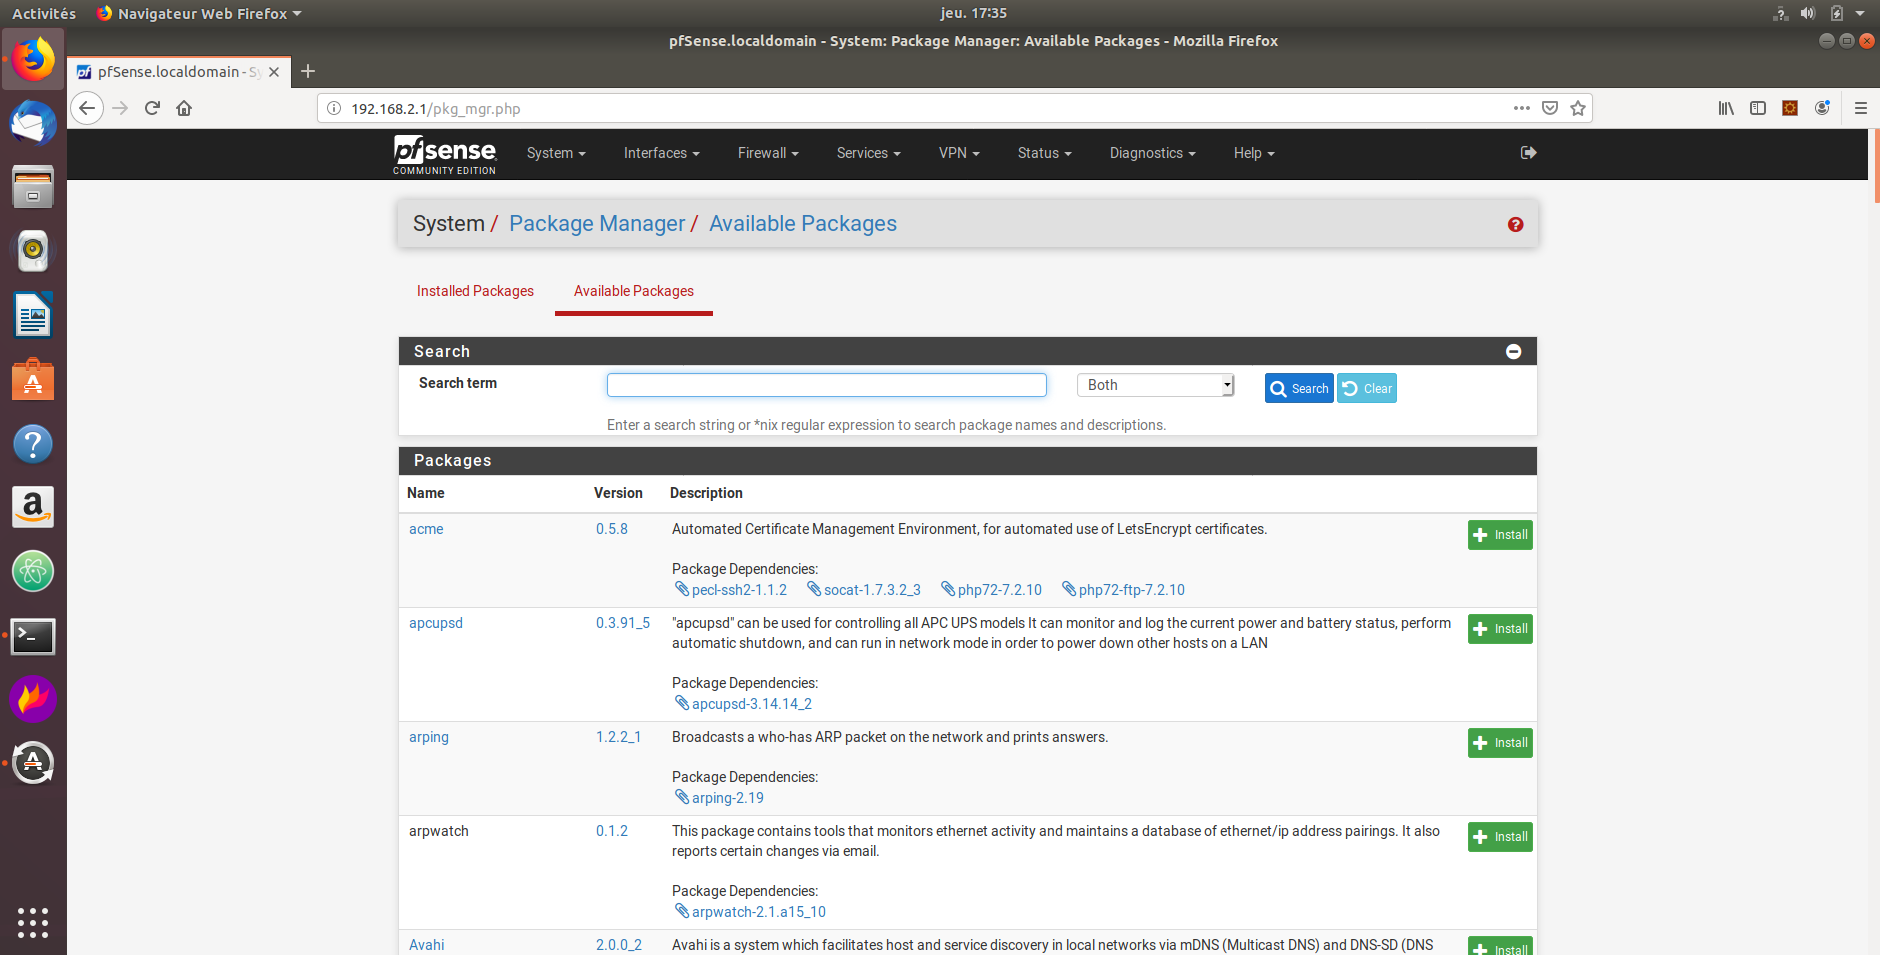
\includegraphics[scale=0.33]{MISP_Screenshots/Snort/2.png}
        \label{MISP_Screenshots/Snort/2}
        \caption{Accès à la recherche de paquet sur Pfsense}
    \end{center}
\end{figure}
\FloatBarrier

Entrer le mot-clé \texttt{snort} dans la barre de recherche de paquets :
\begin{figure}[h!]
    \begin{center}
        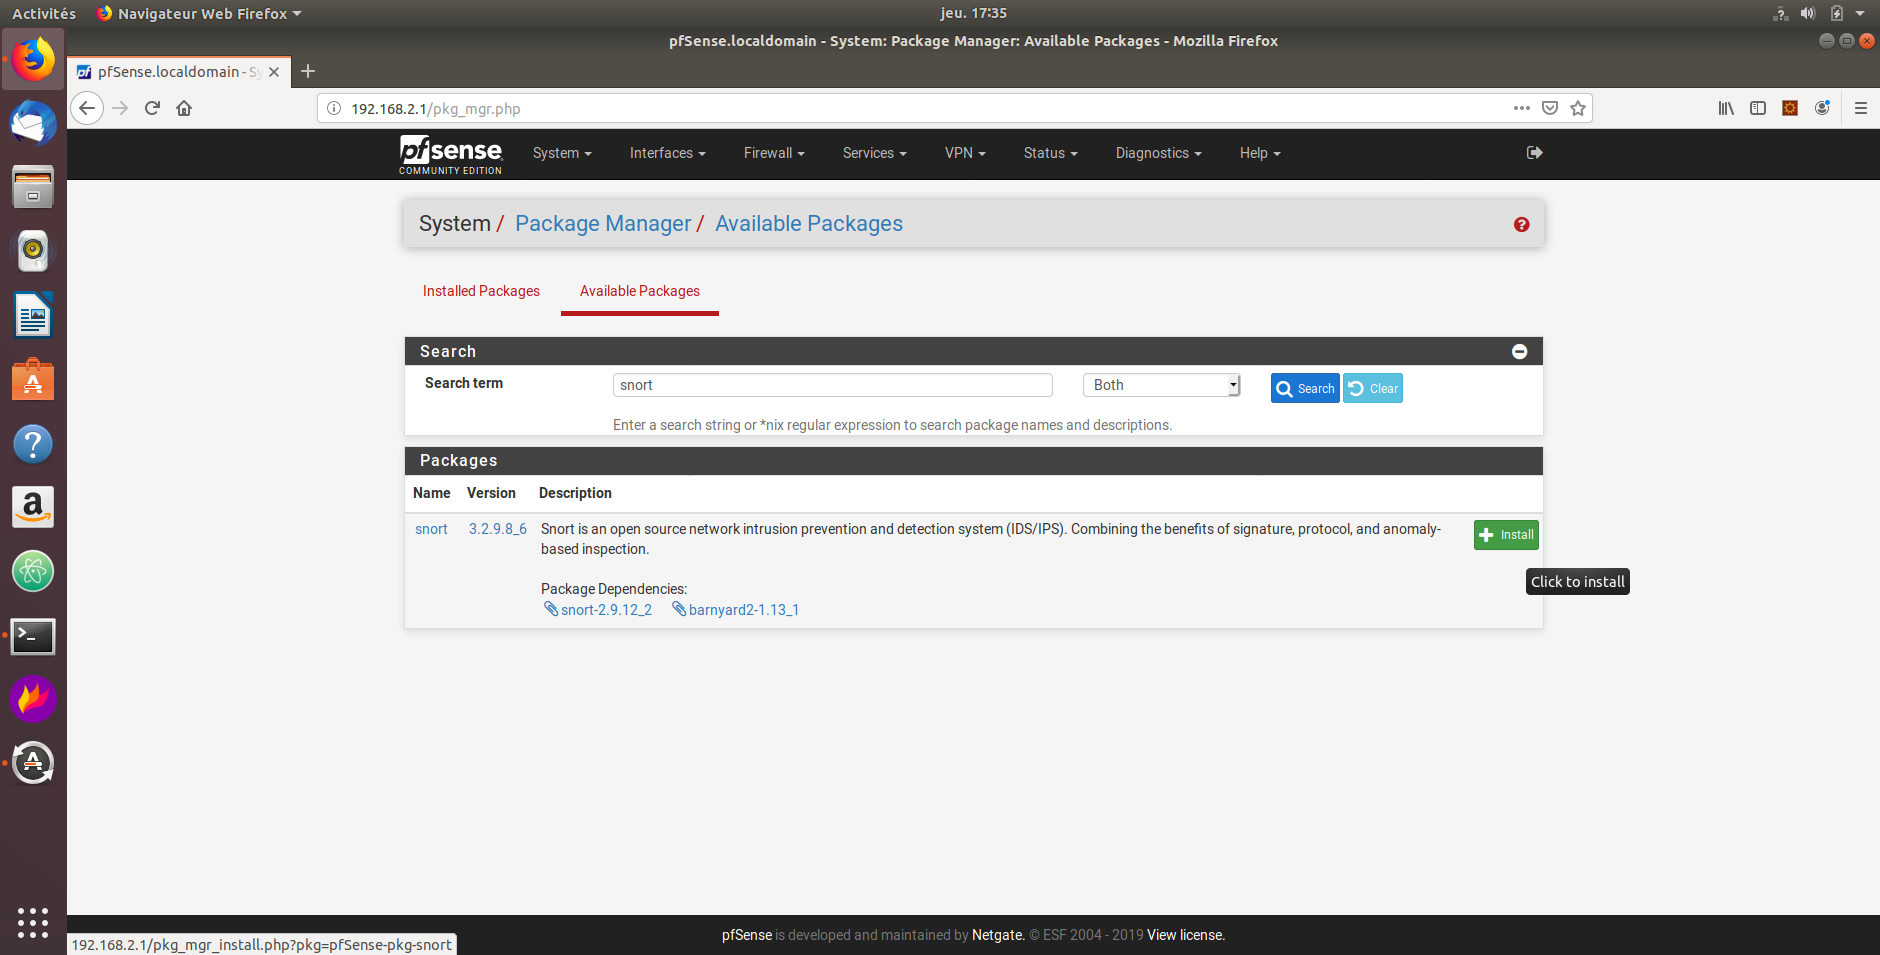
\includegraphics[scale=0.33]{MISP_Screenshots/Snort/3.png}
        \label{MISP_Screenshots/Snort/3}
        \caption{Recherche du package SNORT sur Pfsense}
    \end{center}
\end{figure}
\FloatBarrier

\pagebreak

Confirmer l'installation du paquet, en cliquant sur le bouton \textit{Confirm} :
\begin{figure}[h!]
    \begin{center}
        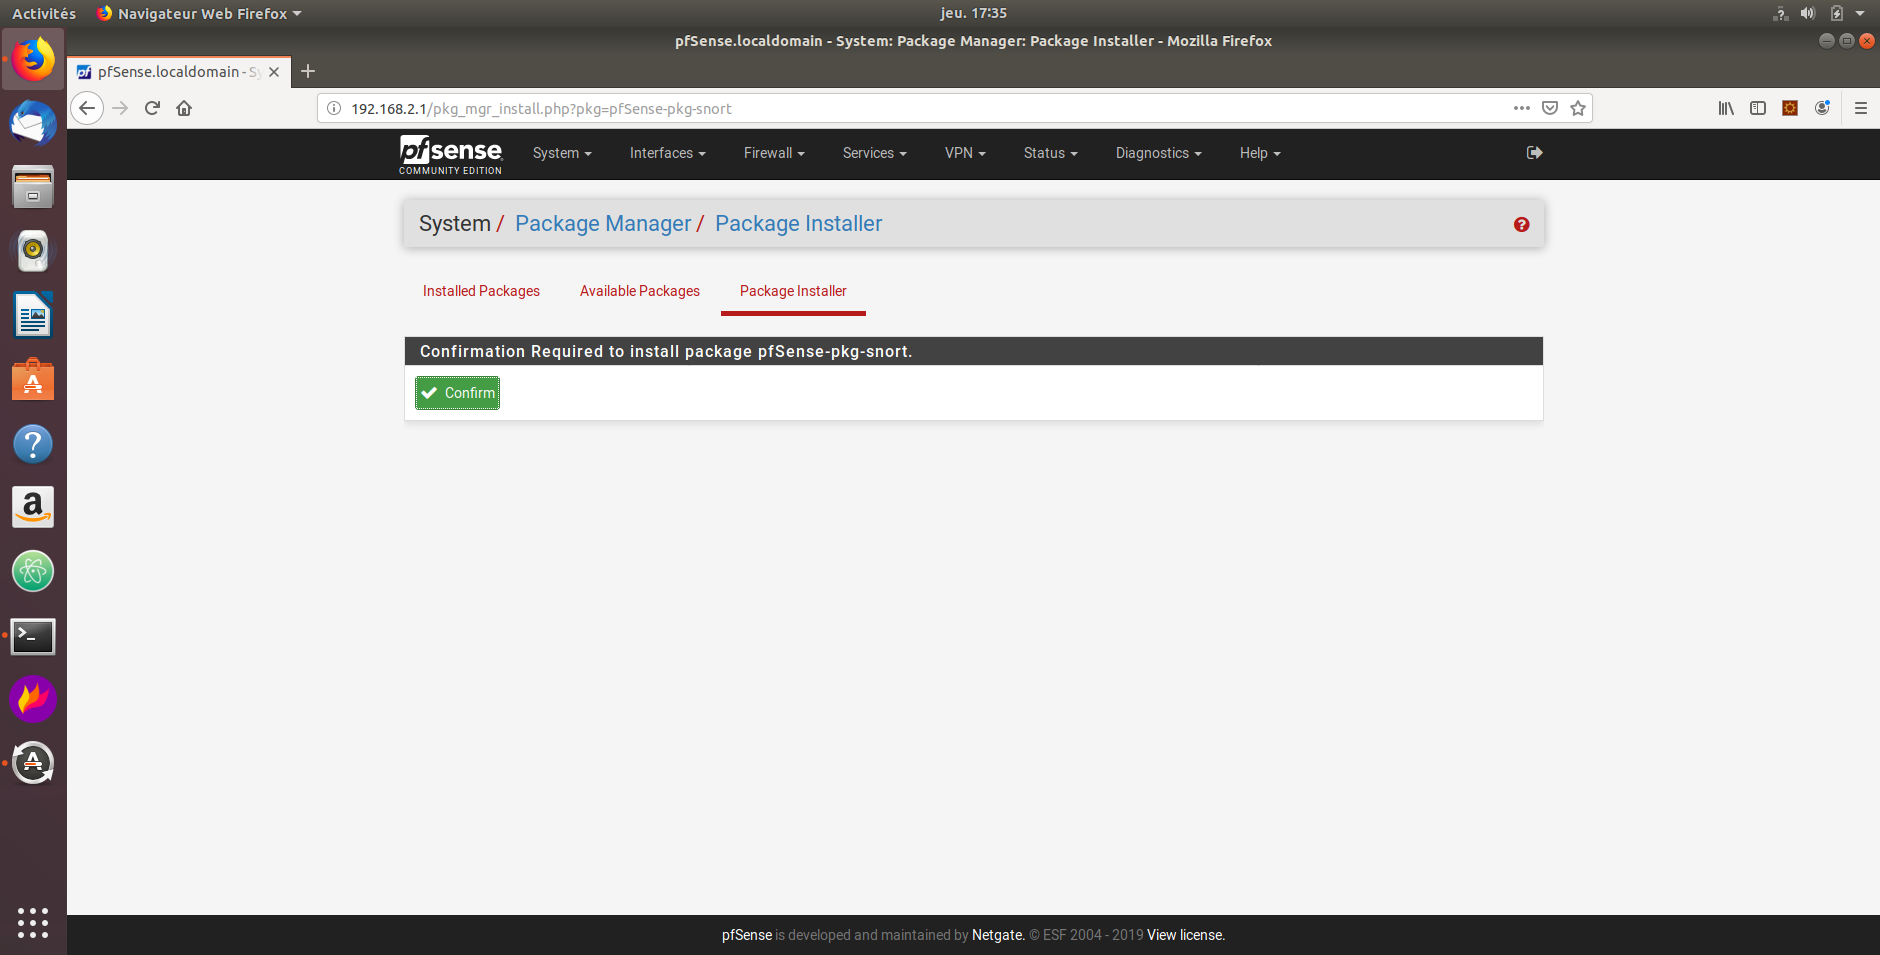
\includegraphics[scale=0.33]{MISP_Screenshots/Snort/4.png}
        \label{MISP_Screenshots/Snort/4}
        \caption{Acceptation du paquet à installer sur Pfsense}
    \end{center}
\end{figure}
\FloatBarrier 
    
Attendre la fin de l'installation du paquet Snort :
\begin{figure}[h!]
    \begin{center}
        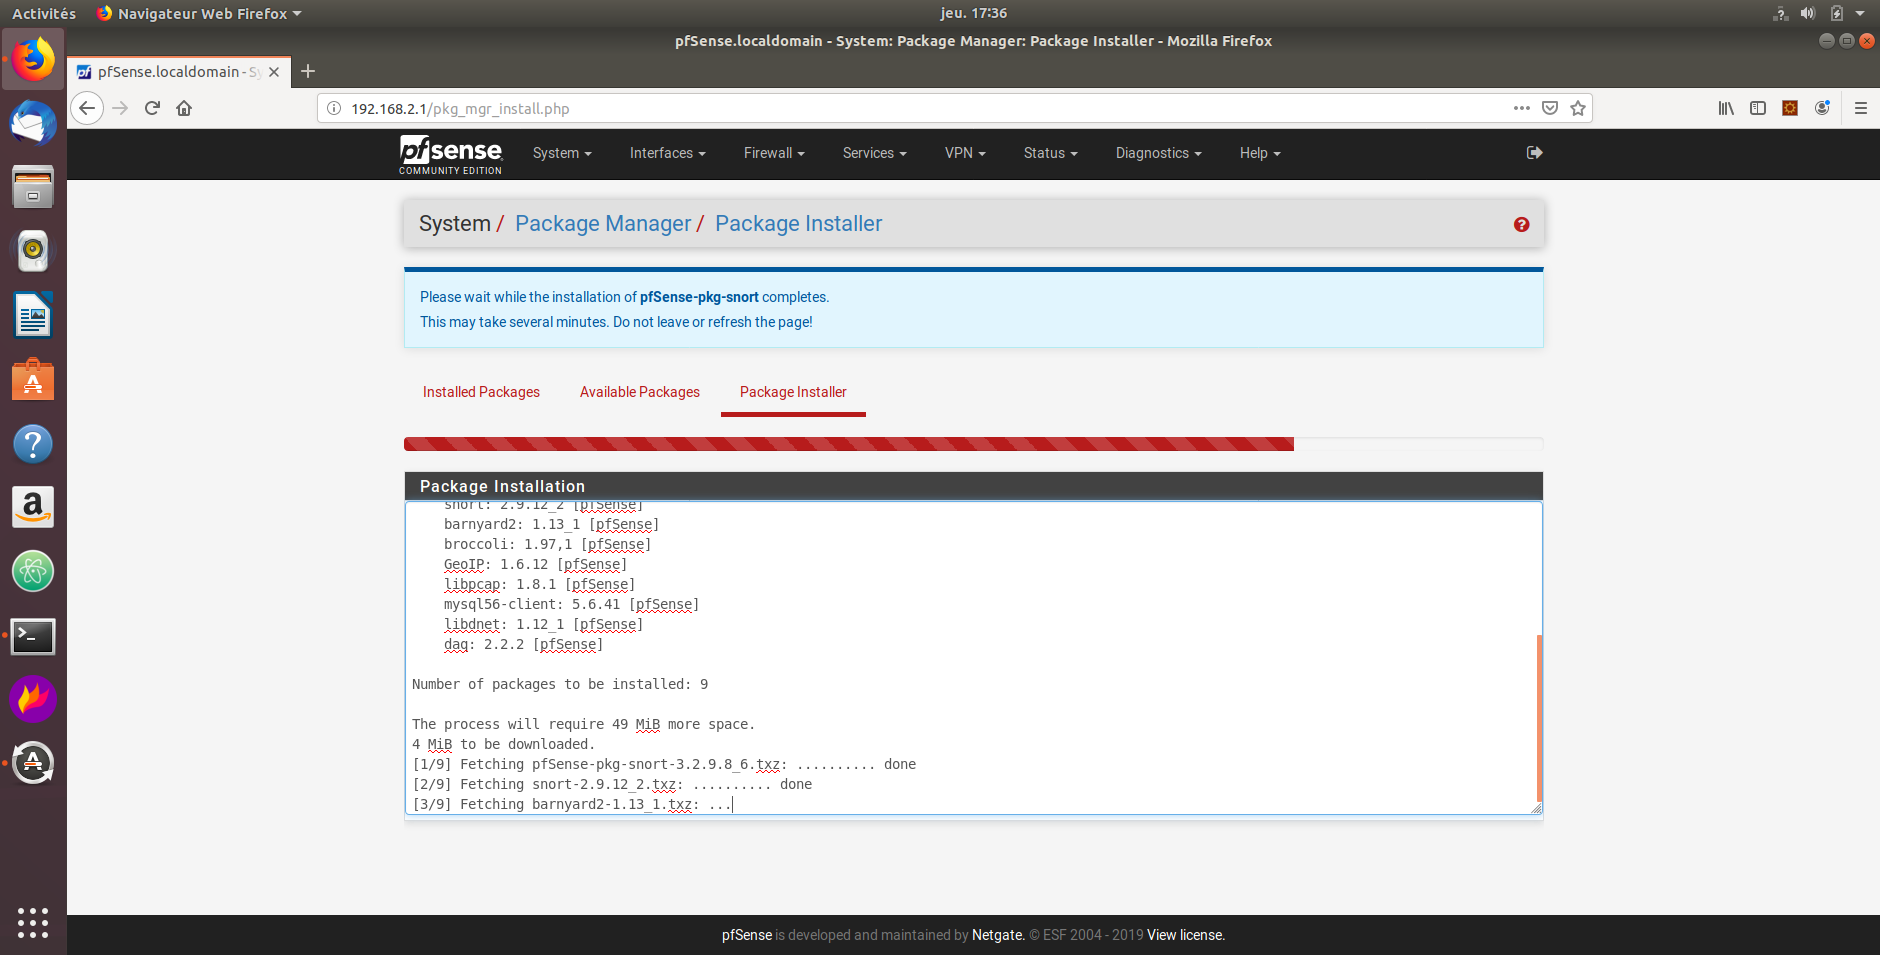
\includegraphics[scale=0.33]{MISP_Screenshots/Snort/5.png}
        \label{MISP_Screenshots/Snort/5}
        \caption{Installation en cours du paquet SNORT sur Pfsense}
    \end{center}
\end{figure}
\FloatBarrier 
    

\begin{figure}[h!]
    \begin{center}
        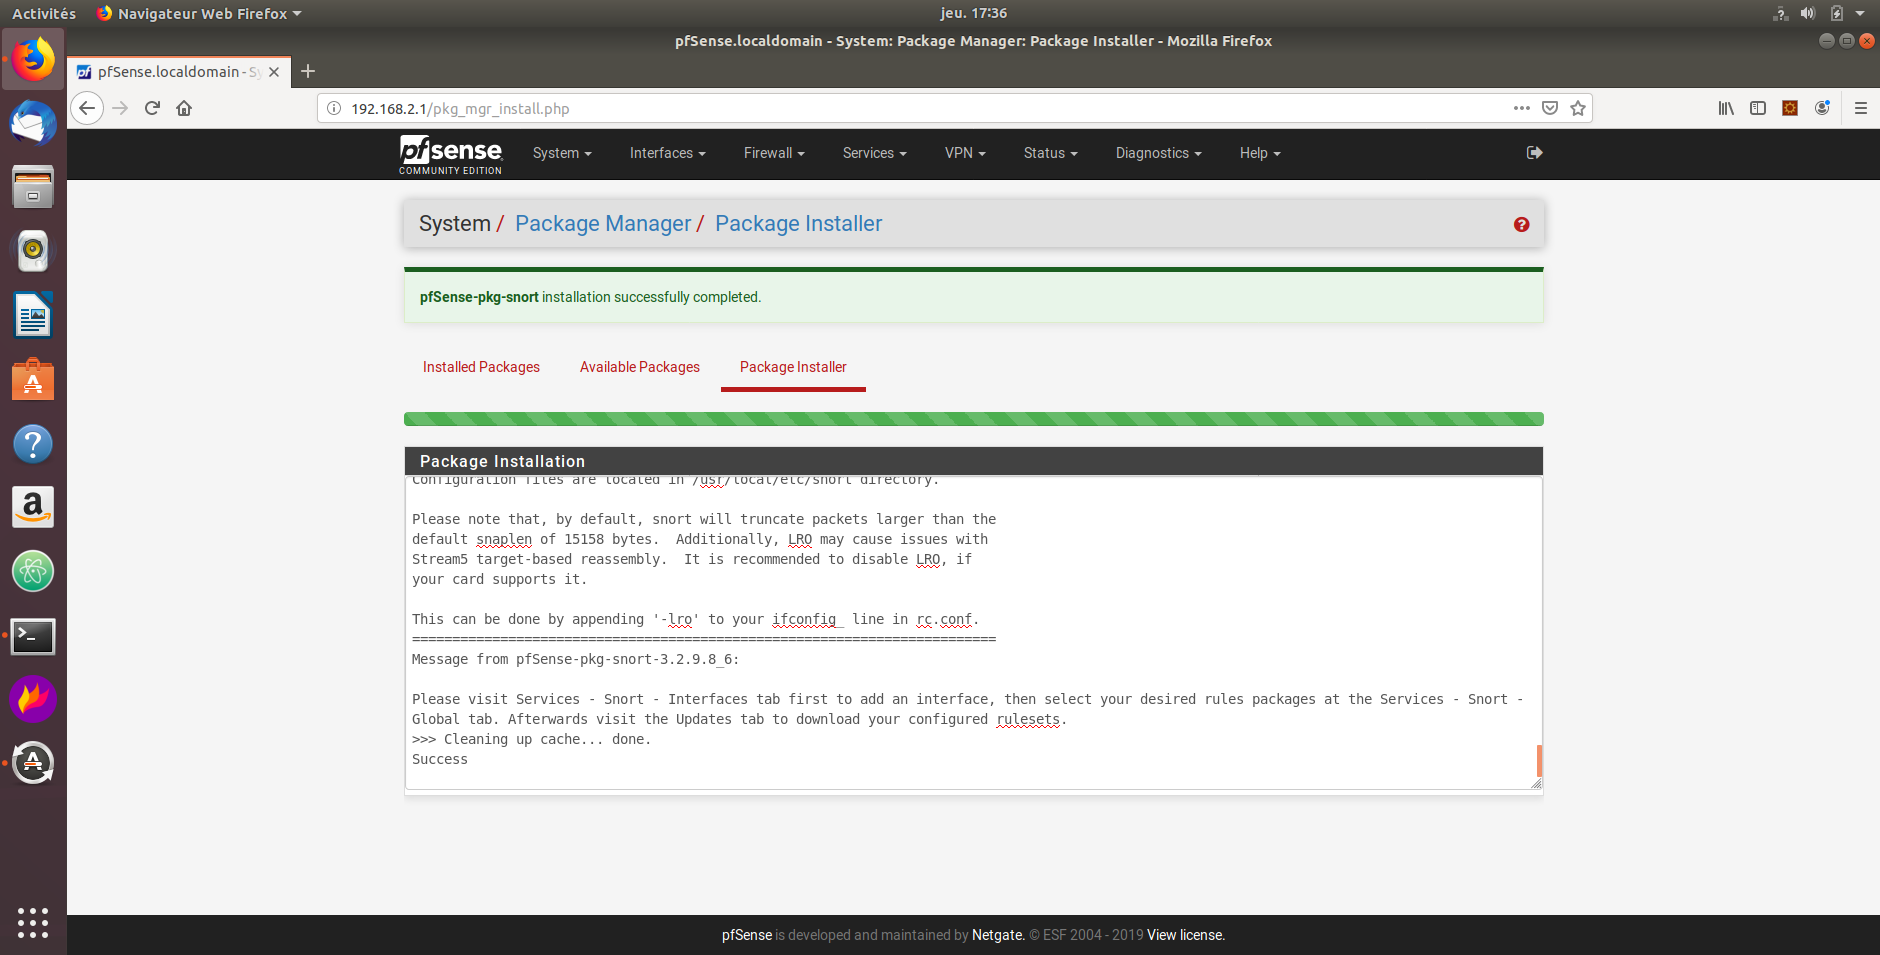
\includegraphics[scale=0.33]{MISP_Screenshots/Snort/6.png}
        \label{MISP_Screenshots/Snort/6}
        \caption{Installation terminée de SNORT sur Pfsense}
    \end{center}
\end{figure}
\FloatBarrier 

Afin d'accéder à la page du service Snort sur l'interface web de Pfsense, cliquer sur l'onglet \textbf{Services}, puis sur \textit{Snort} :
\begin{figure}[h!]
    \begin{center}
        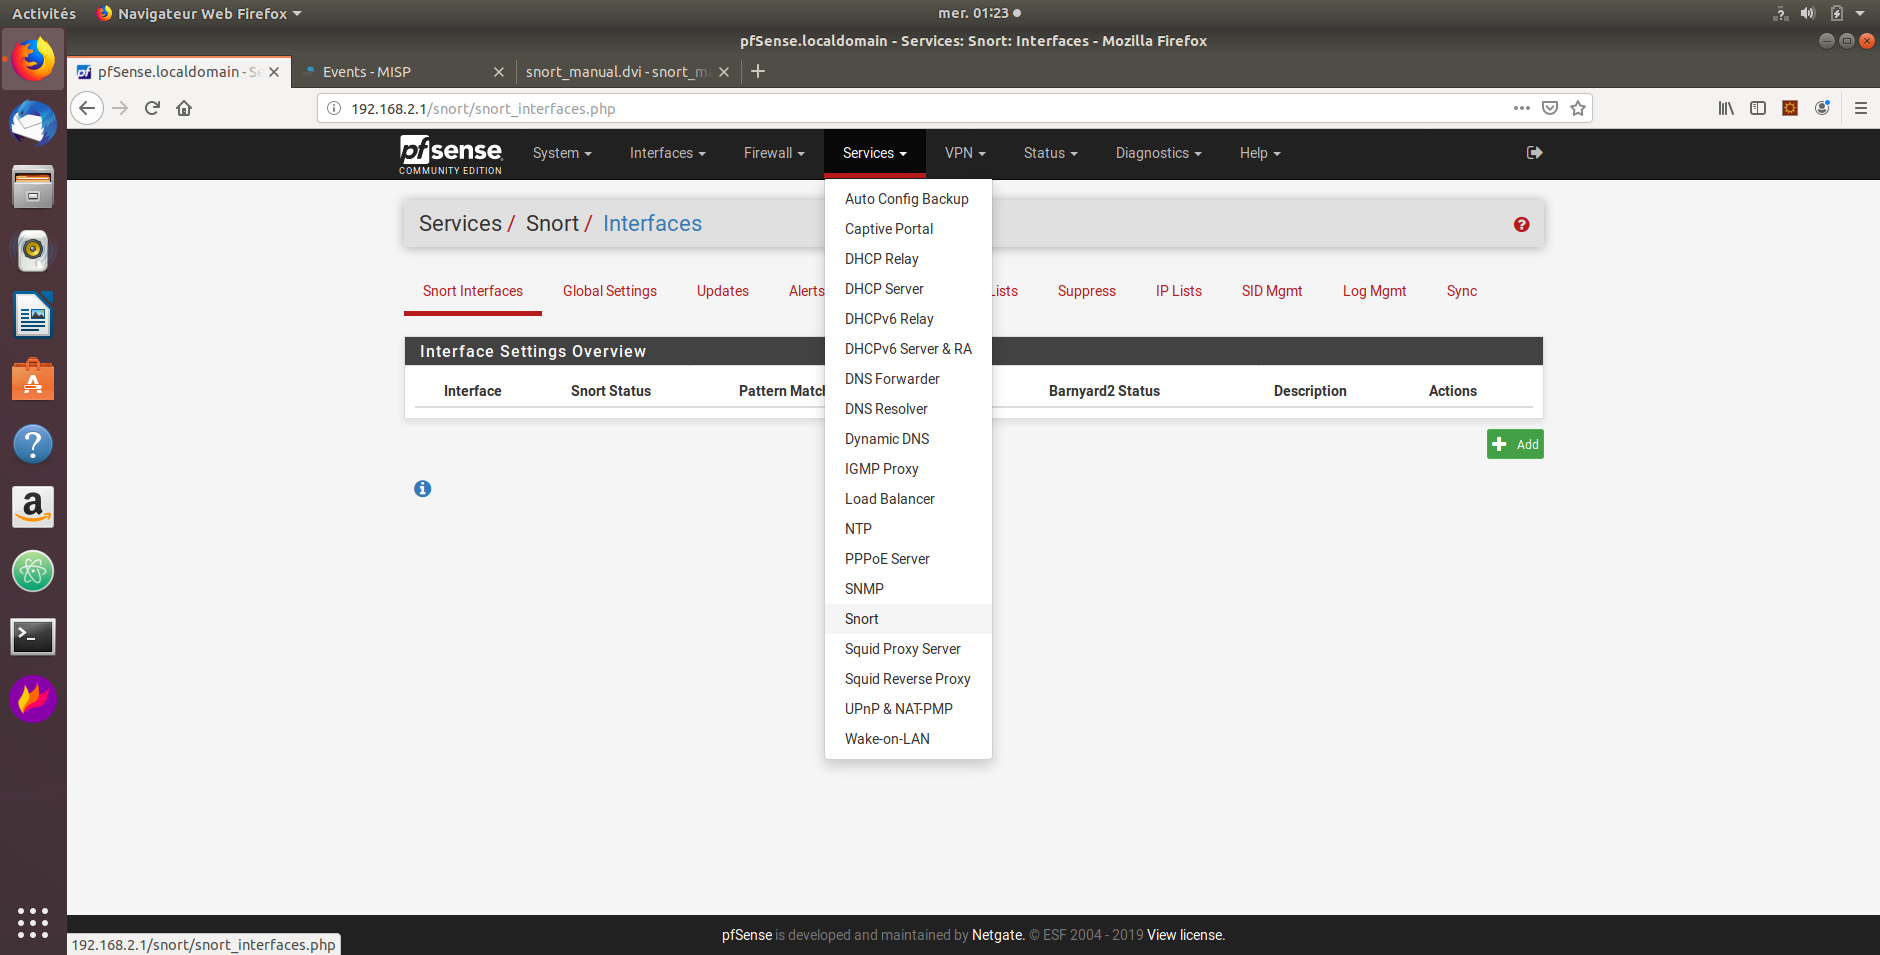
\includegraphics[scale=0.33]{MISP_Screenshots/Snort/7.png}
        \label{MISP_Screenshots/Snort/7}
        \caption{Accès au service SNORT sur Pfsense}
    \end{center}
\end{figure}
\FloatBarrier

\pagebreak

Ajouter une nouvelle interface WAN en cliquant sur le bouton \textit{Add} :
\begin{figure}[h!]
    \begin{center}
        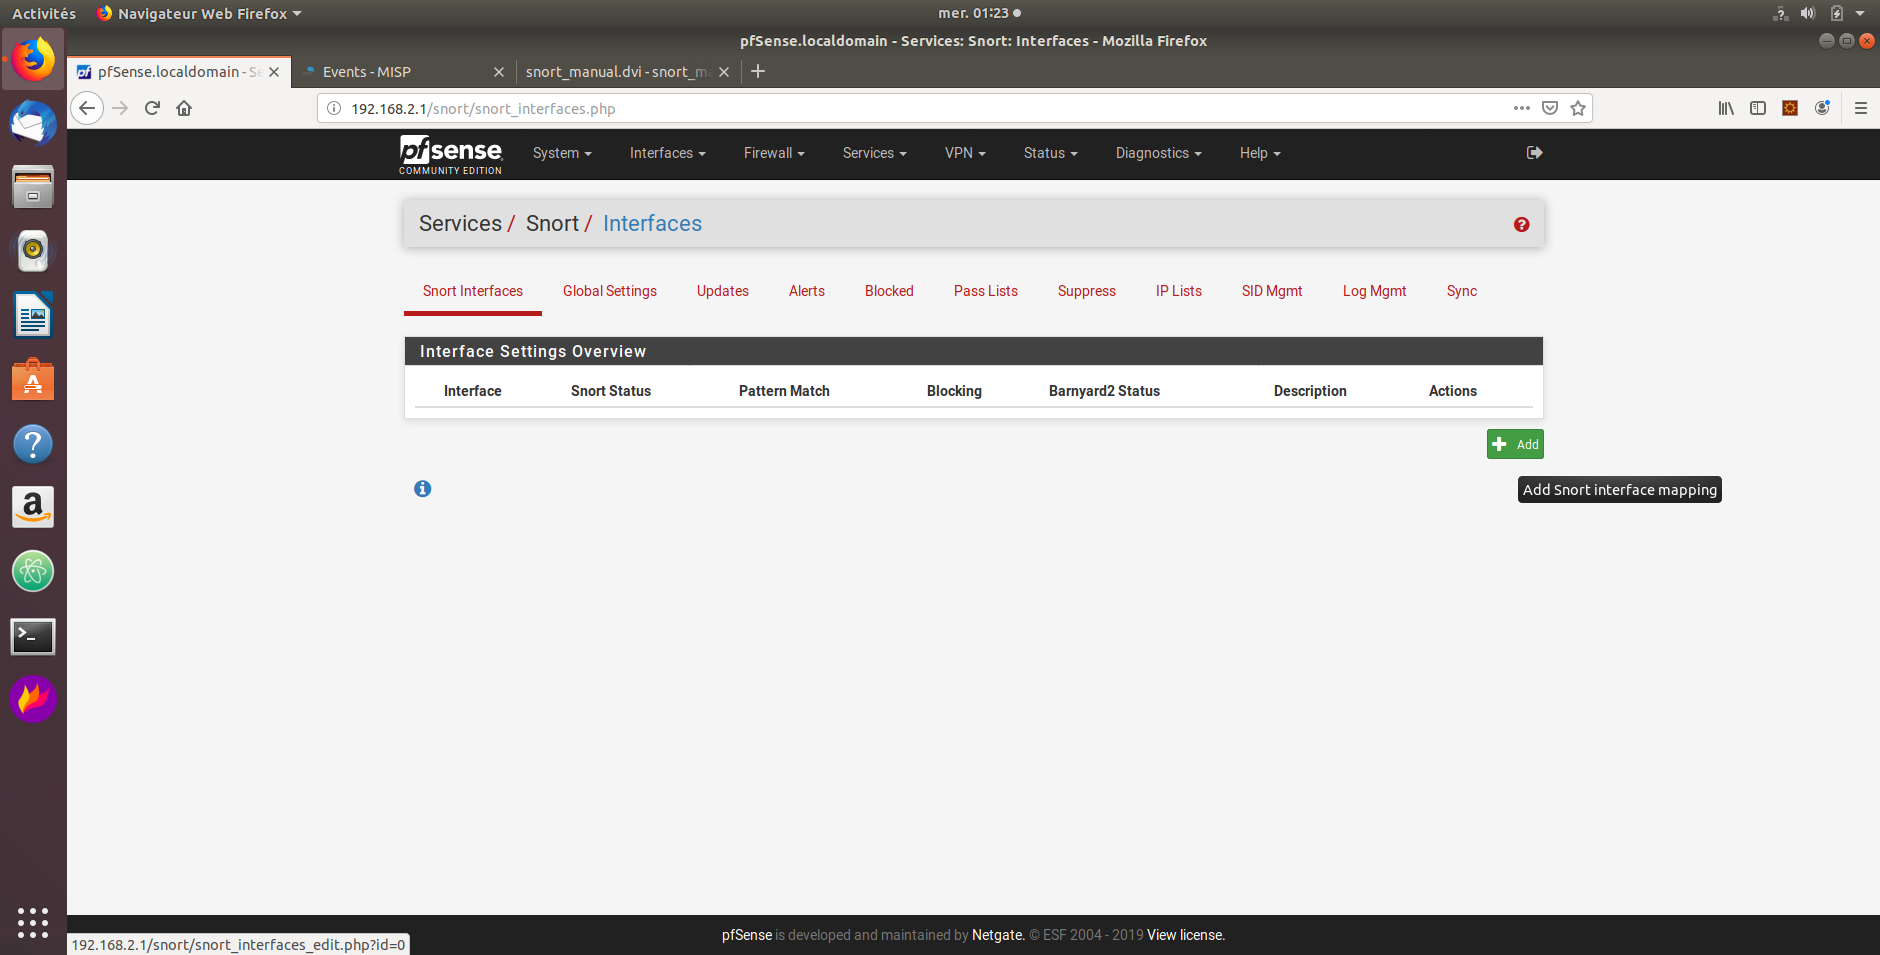
\includegraphics[scale=0.33]{MISP_Screenshots/Snort/8.png}
        \label{MISP_Screenshots/Snort/8}
        \caption{Ajout d'une nouvelle interface WAN via SNORT}
    \end{center}
\end{figure}
\FloatBarrier 

Configurer l'interface WAN, selon la capture d'écran suivante :
\begin{figure}[h!]
    \begin{center}
        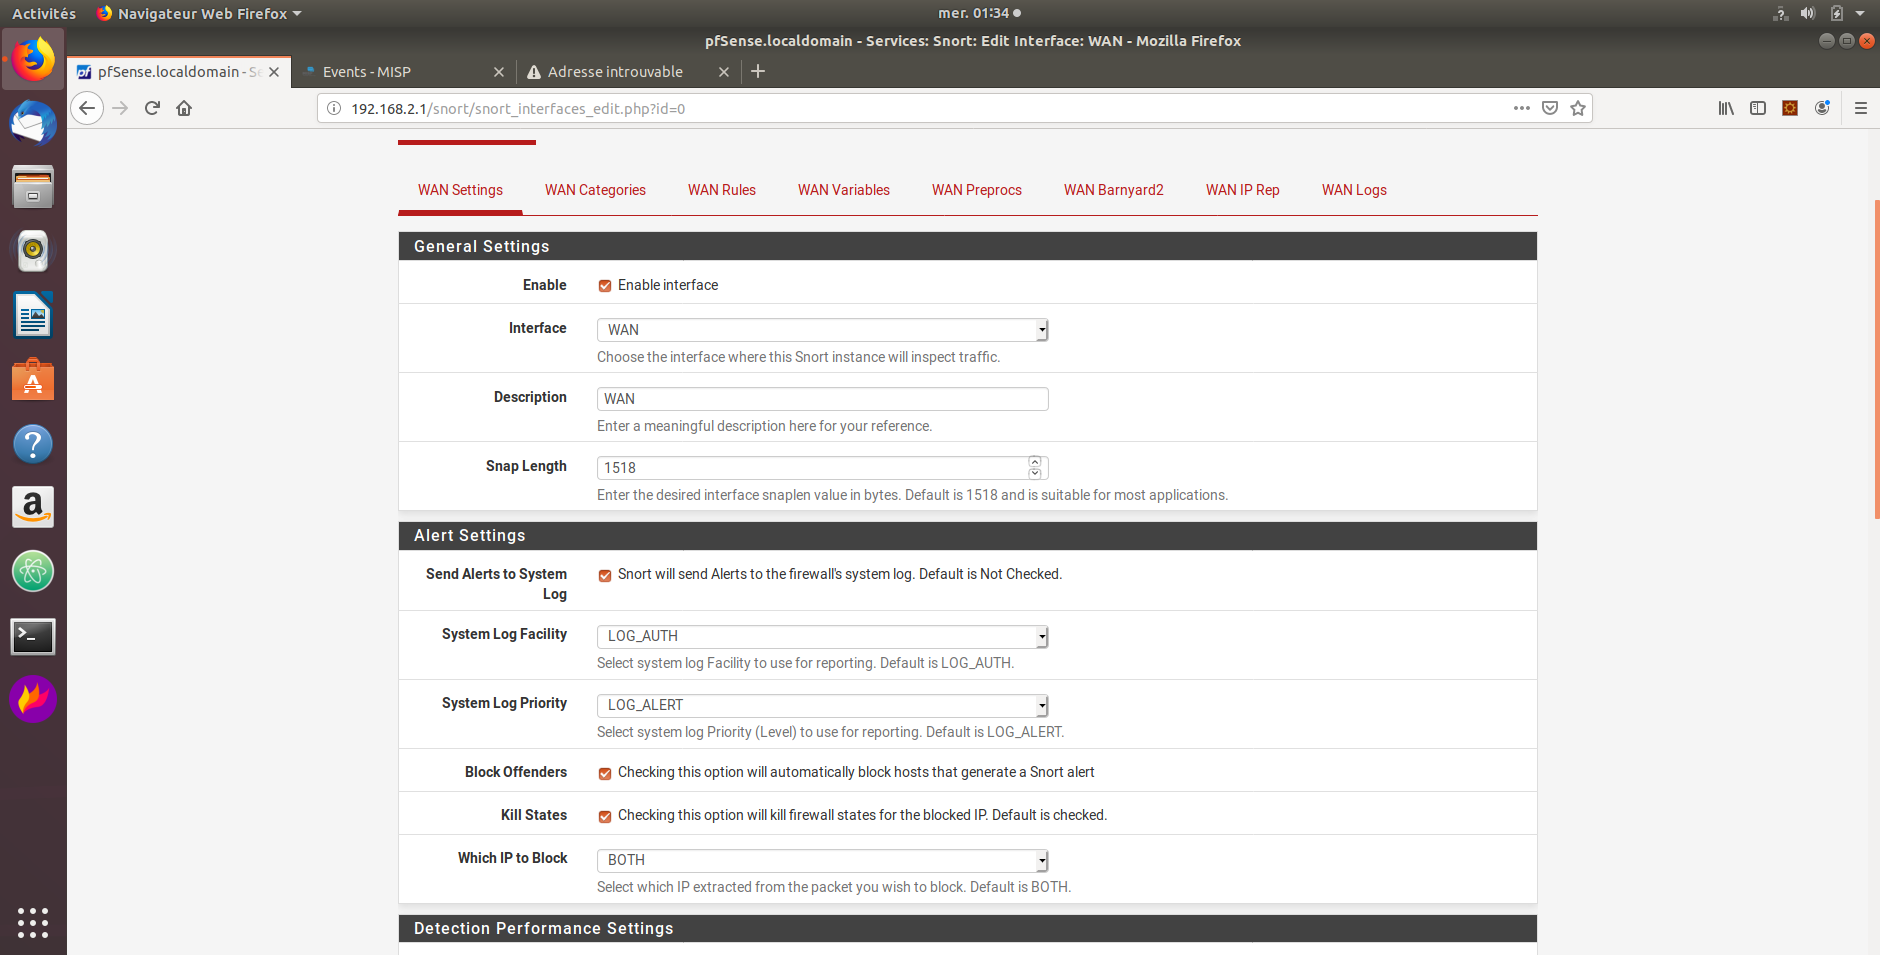
\includegraphics[scale=0.33]{MISP_Screenshots/Snort/9.png}
        \label{MISP_Screenshots/Snort/9}
        \caption{Configuration de la nouvelle interface sur SNORT}
    \end{center}
\end{figure}
\FloatBarrier

\pagebreak

Ajouter le chemin d'un fichier de configuration dans l'encadré \texttt{Advanced Configuration Pass-Through}. Le texte à écrire est donc : \textit{include /usr/local/etc/snort/rules/misp.rules} :
\begin{figure}[h!]
    \begin{center}
        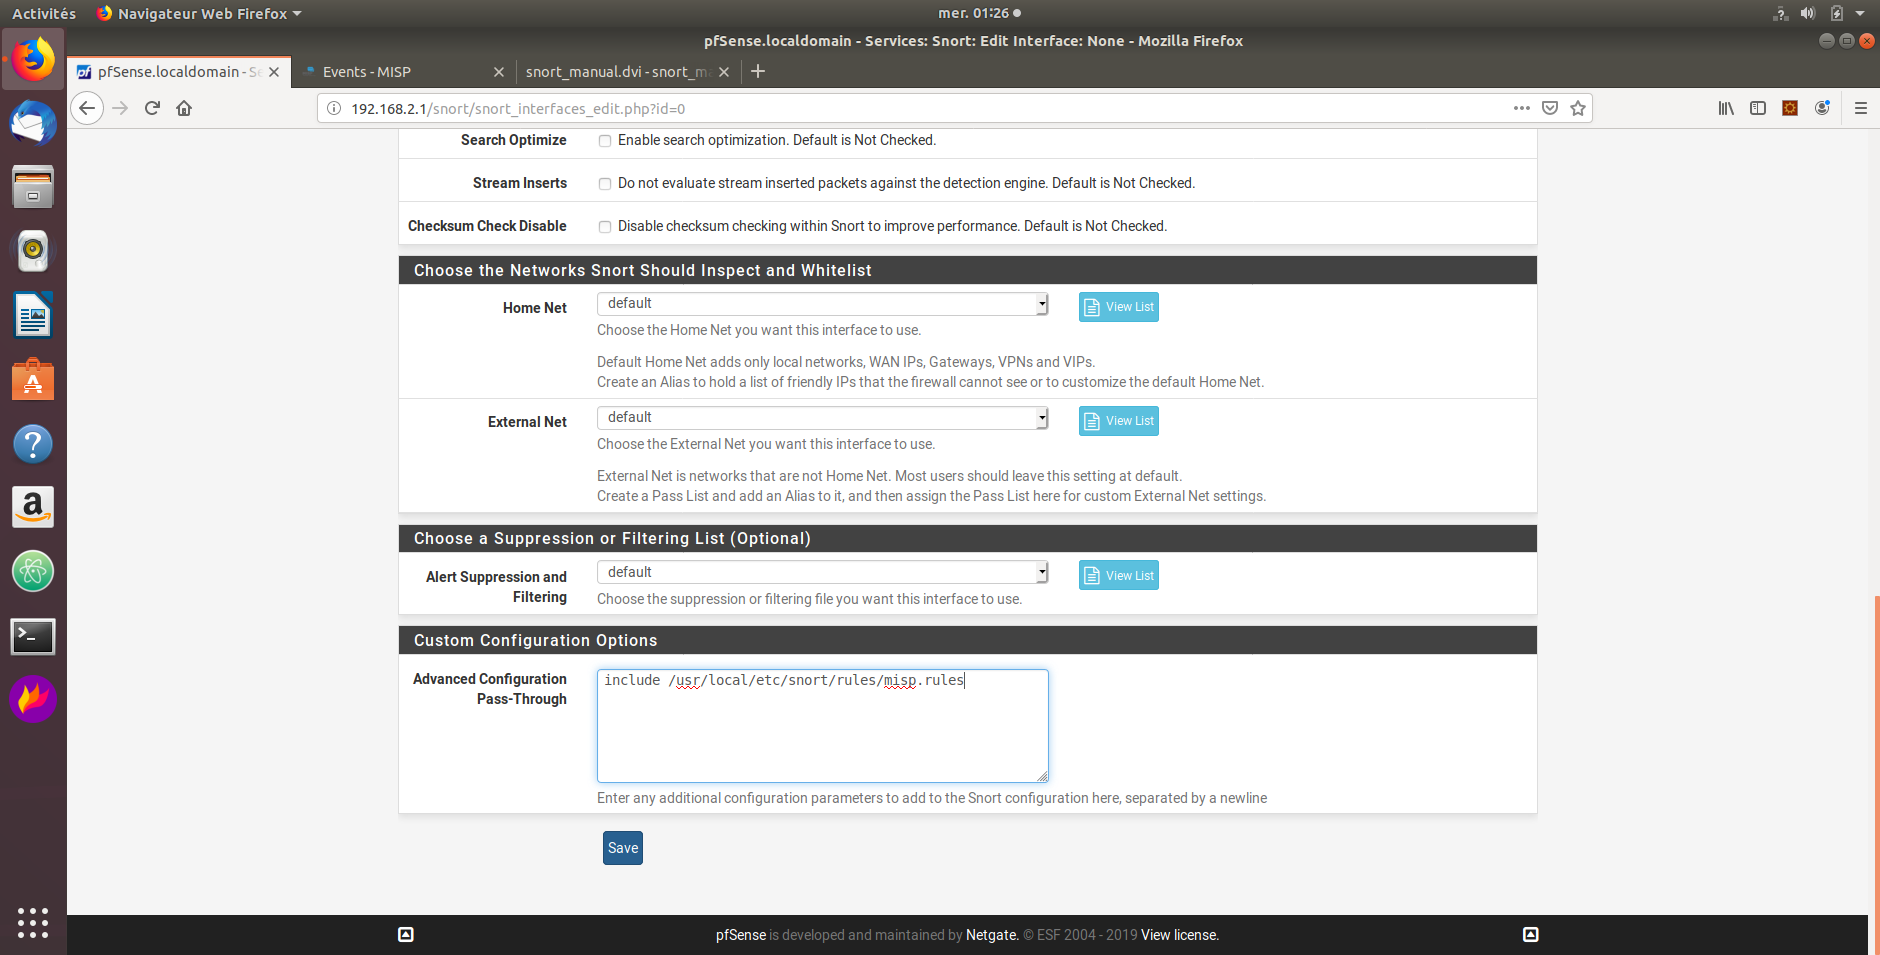
\includegraphics[scale=0.31]{MISP_Screenshots/Snort/10.png}
        \label{MISP_Screenshots/Snort/10}
        \caption{Configuration du fichier incluant les règles SNORT}
    \end{center}
\end{figure}
\FloatBarrier 

Dupliquer la configuration de l'interface WAN pour faire une interface LAN :
\begin{figure}[h!]
    \begin{center}
        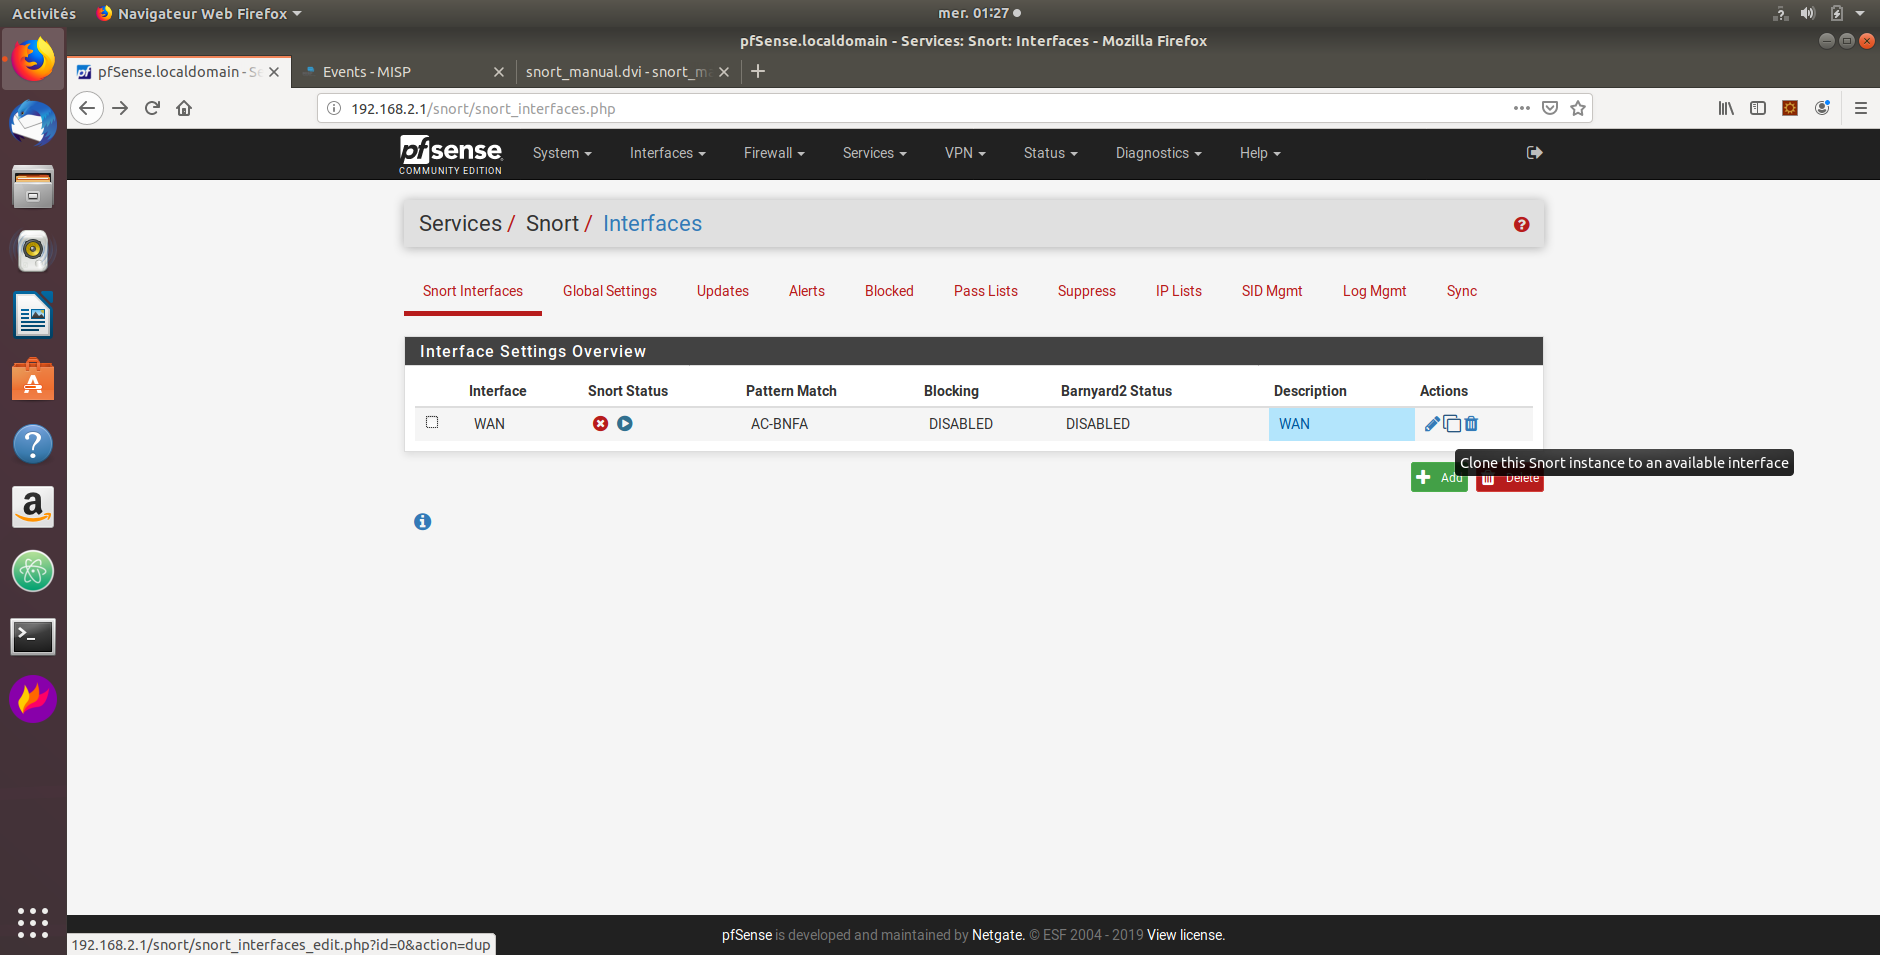
\includegraphics[scale=0.31]{MISP_Screenshots/Snort/11.png}
        \label{MISP_Screenshots/Snort/11}
        \caption{Duplication de la configuration SNORT pour le LAN}
    \end{center}
\end{figure}
\FloatBarrier

\pagebreak

Configurer la nouvelle interface LAN, tel que sur la capture d'écran suivante :
\begin{figure}[h!]
    \begin{center}
        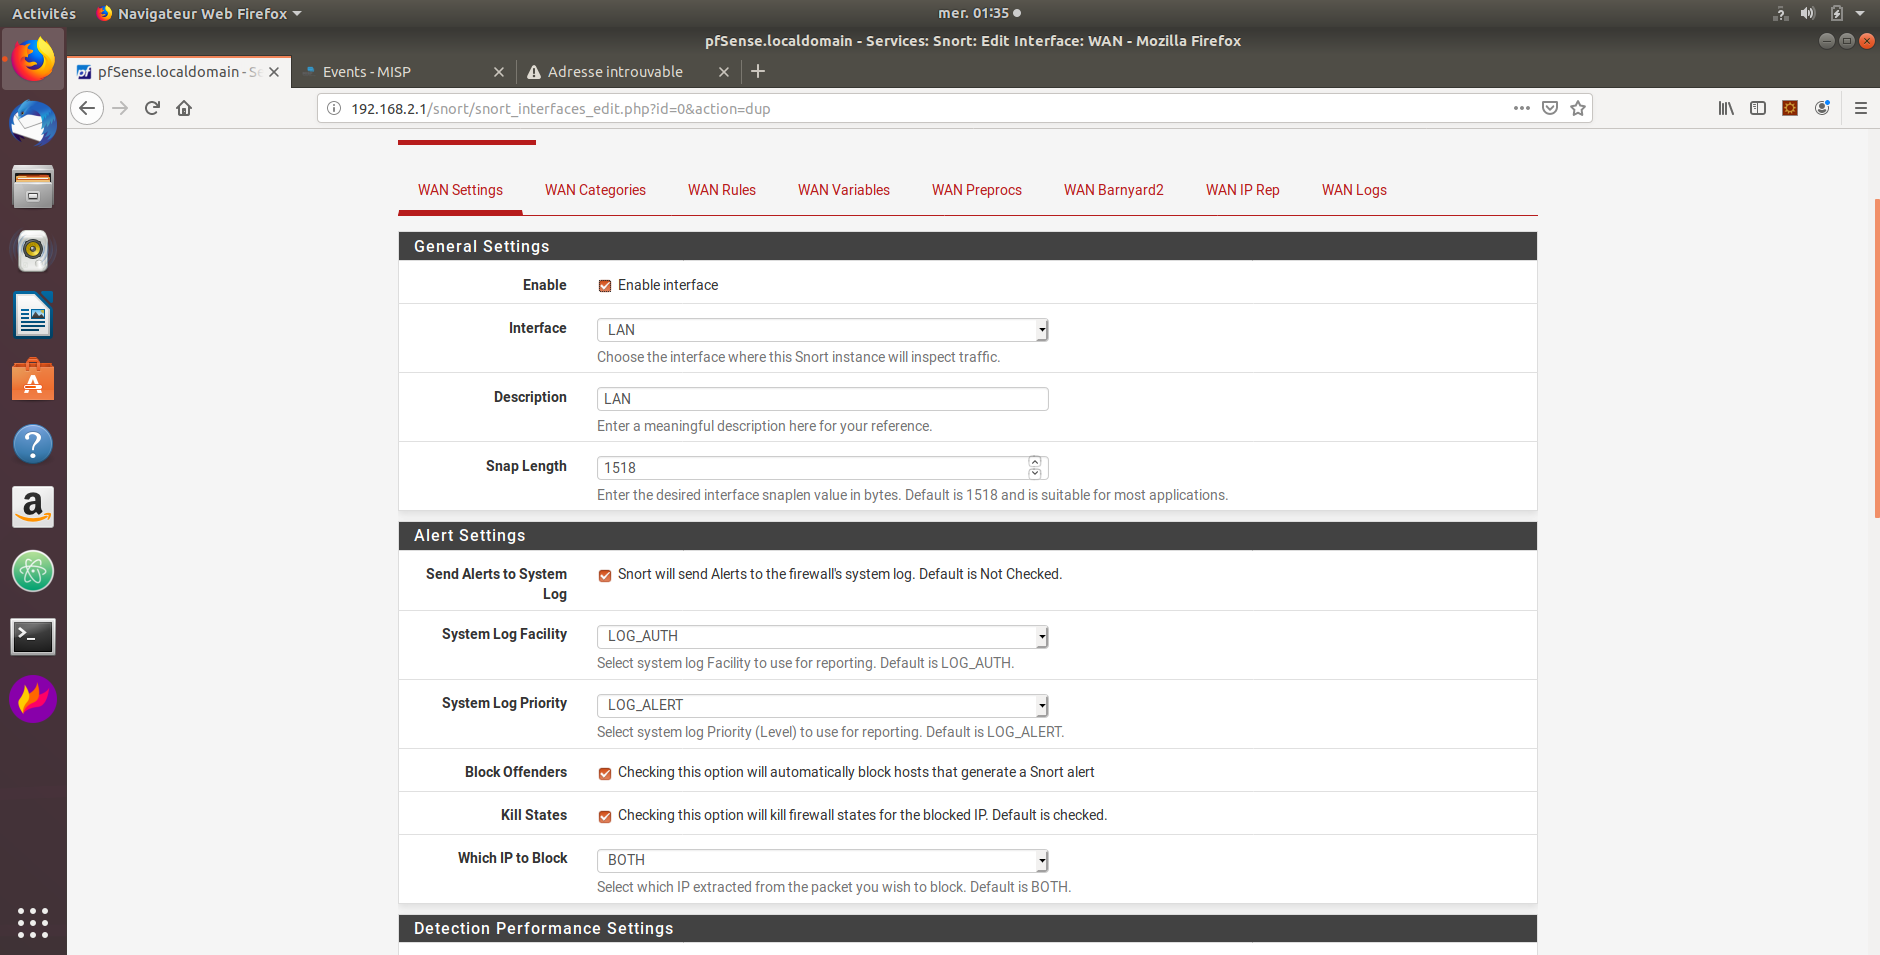
\includegraphics[scale=0.33]{MISP_Screenshots/Snort/12.png}
        \label{MISP_Screenshots/Snort/12}
        \caption{Configuration de la nouvelle interface LAN sur SNORT}
    \end{center}
\end{figure}
\FloatBarrier

Comme pour l'interface WAN, ajouter le chemin du fichier de configuration dans l'encadré \texttt{Advanced Configuration Pass-Through} : \textit{include/usr/local/etc/snort/rules/misp.rules} :
\begin{figure}[h!]
    \begin{center}
        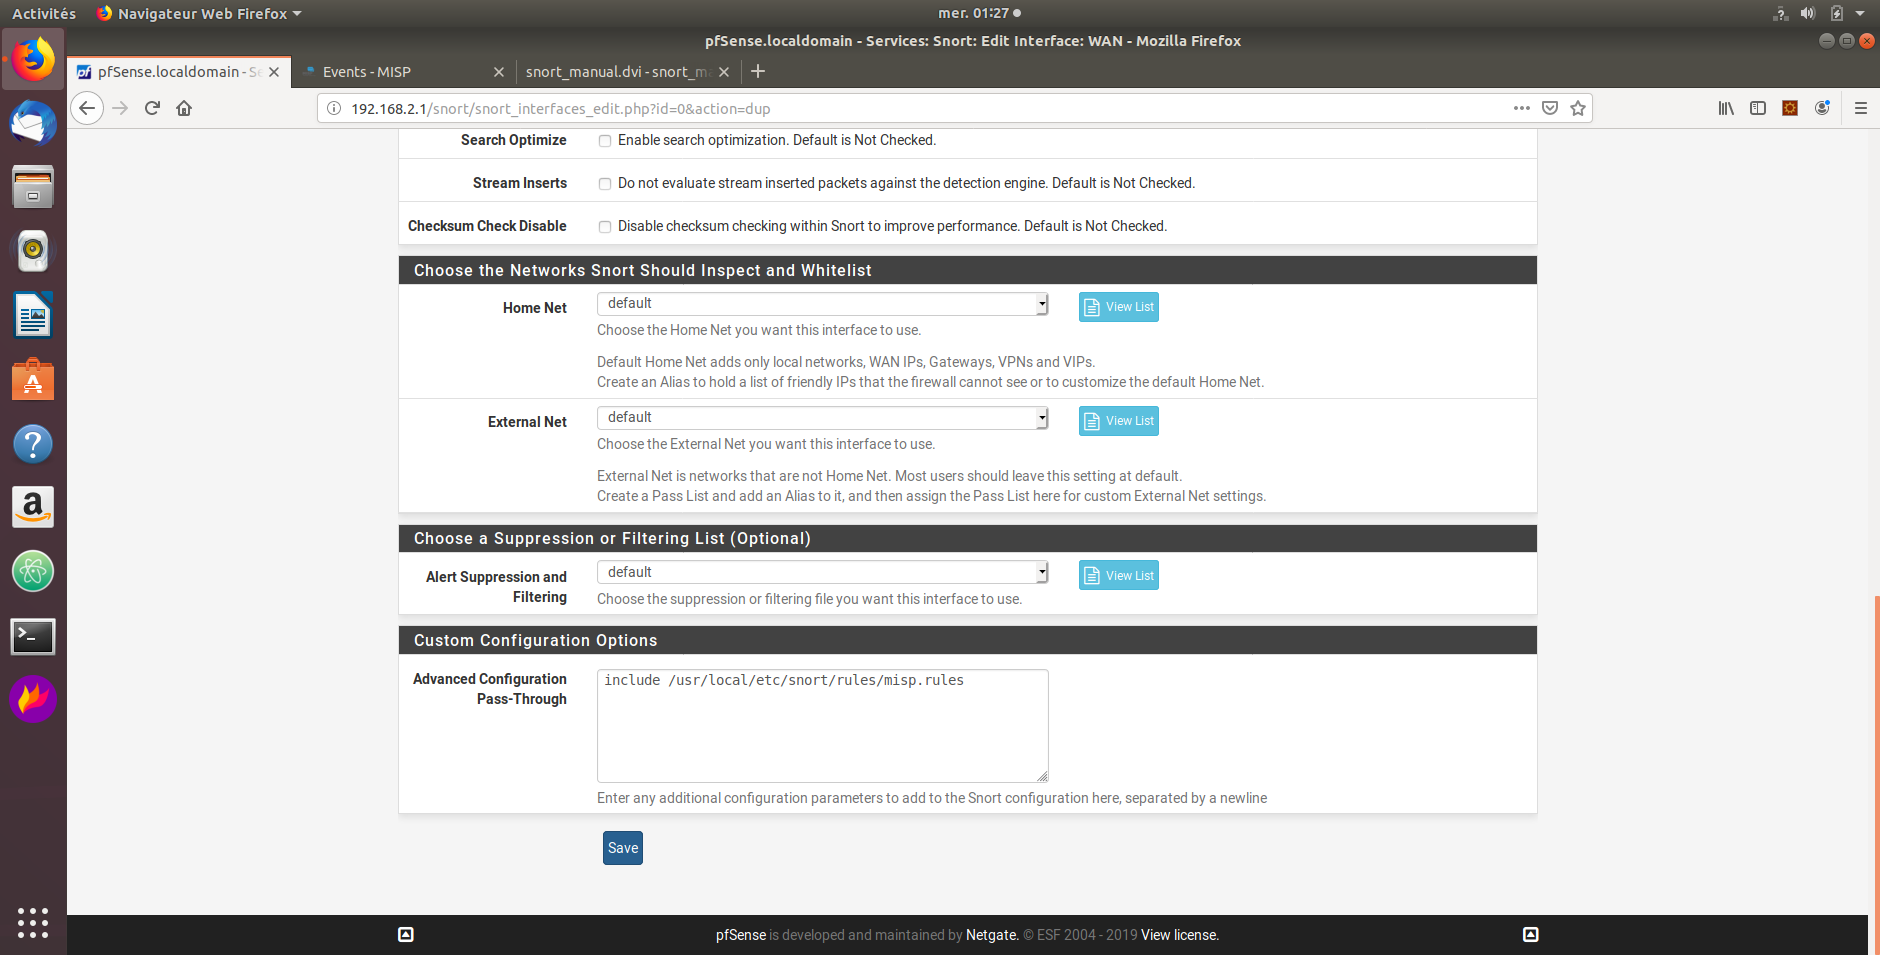
\includegraphics[scale=0.31]{MISP_Screenshots/Snort/13.png}
        \label{MISP_Screenshots/Snort/13}
        \caption{Configuration du fichier incluant les règles SNORT sur le LAN}
    \end{center}
\end{figure}
\FloatBarrier

\pagebreak

De la même manière que pour les interfaces WAN et LAN, créer une nouvelle interface pour la DMZ :
\begin{figure}[h!]
    \begin{center}
        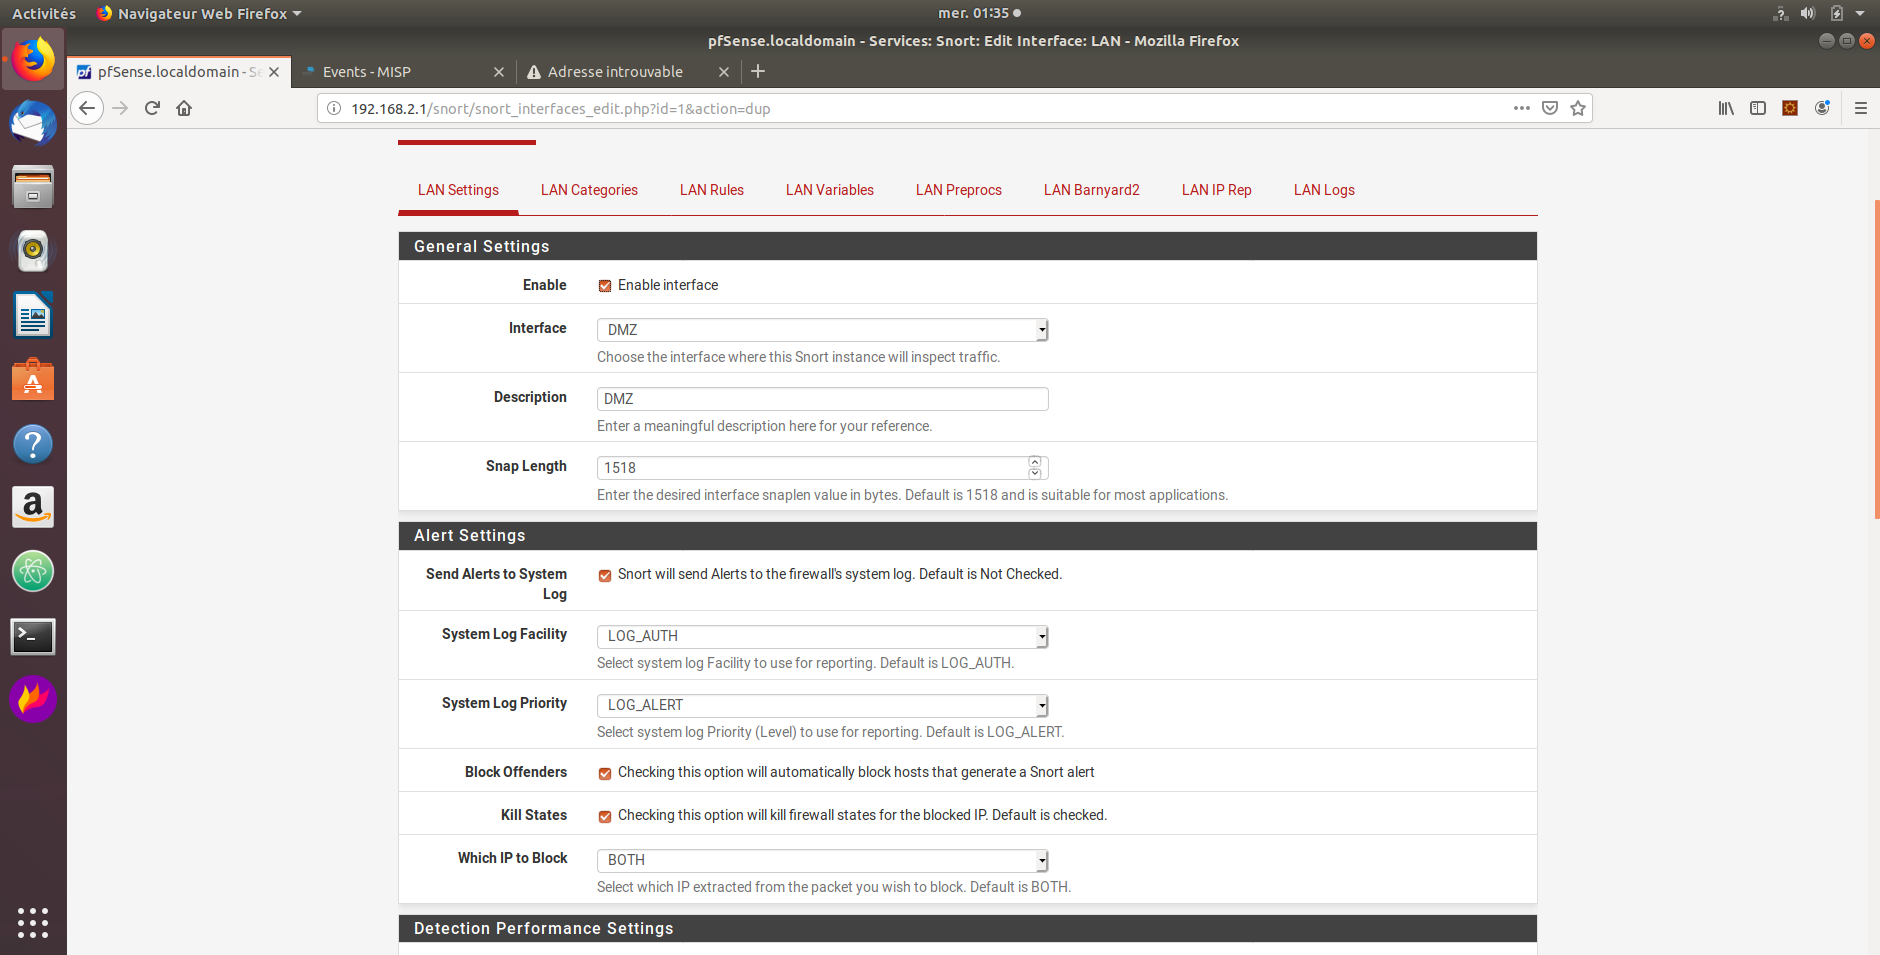
\includegraphics[scale=0.31]{MISP_Screenshots/Snort/14.png}
        \label{MISP_Screenshots/Snort/14}
        \caption{Configuration de la nouvelle interface DMZ sur SNORT}
    \end{center}
\end{figure}
\FloatBarrier 

Encore une fois, ajouter le chemin du fichier de configuration dans l'encadré \texttt{Advanced Configuration Pass-Through} : \textit{include /usr/local/etc/snort/rules/misp.rules} :
\begin{figure}[h!]
    \begin{center}
        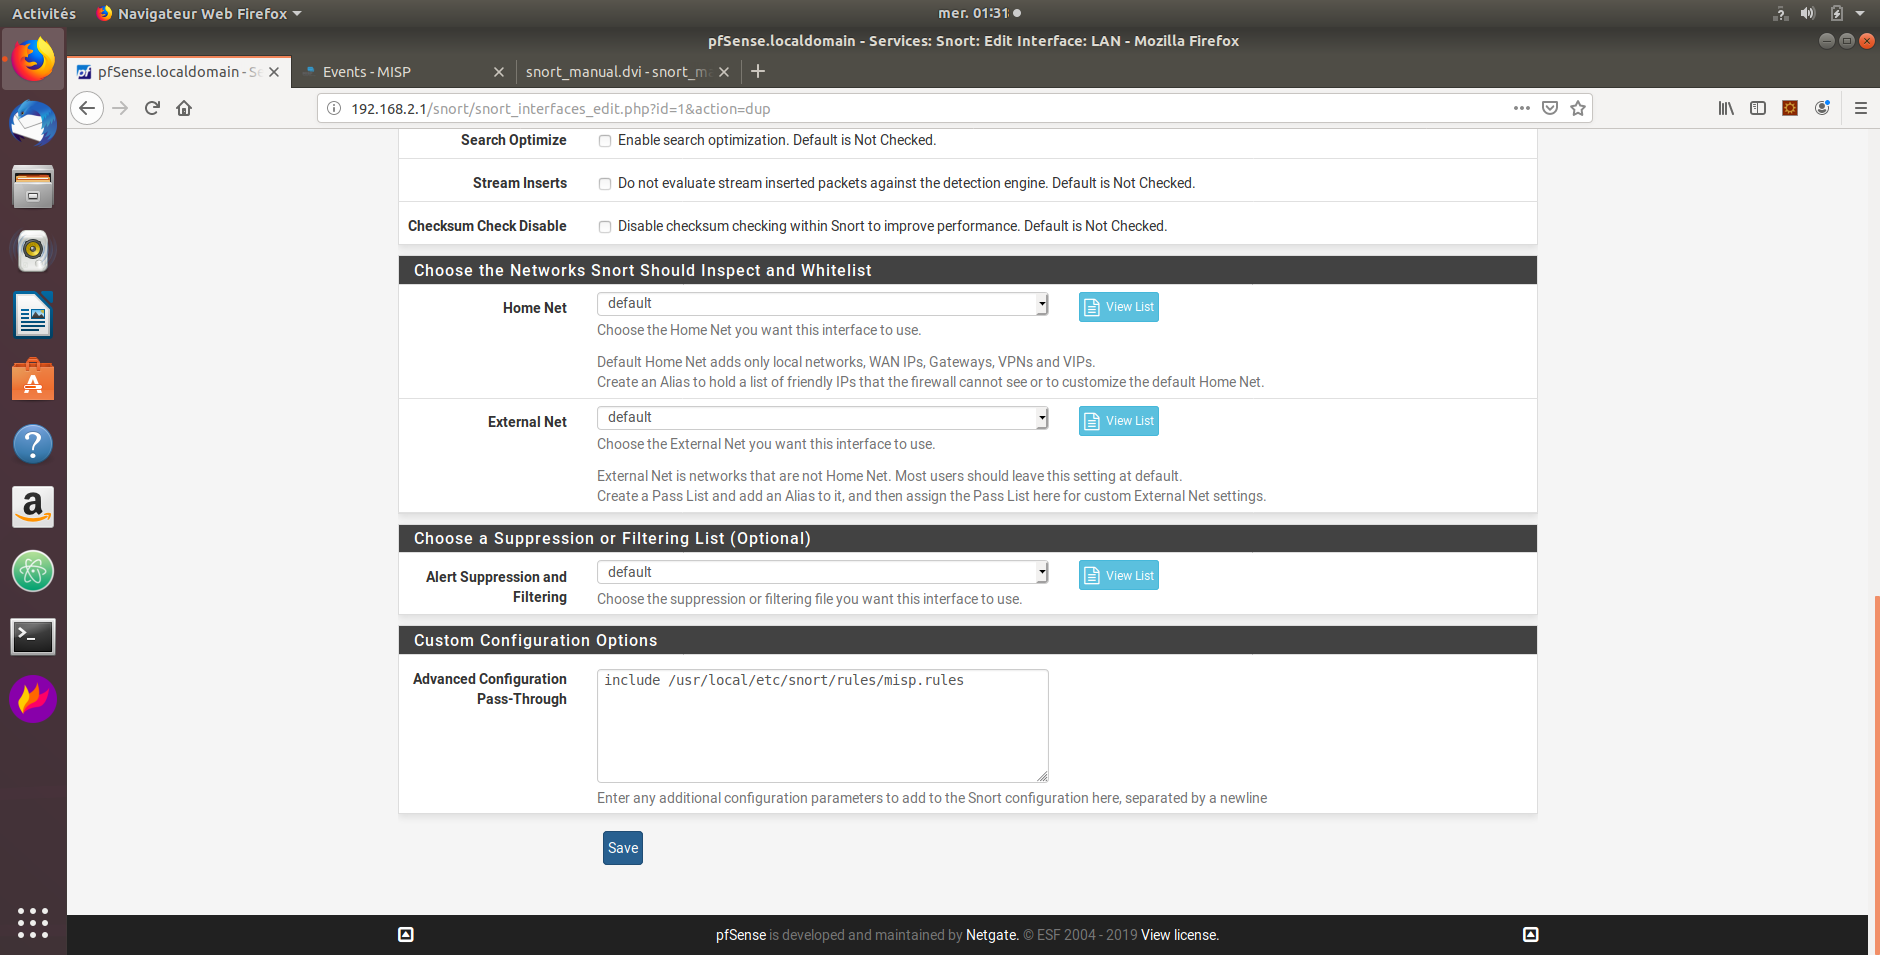
\includegraphics[scale=0.31]{MISP_Screenshots/Snort/15.png}
        \label{MISP_Screenshots/Snort/15}
        \caption{Configuration du fichier incluant les règles SNORT sur la DMZ}
    \end{center}
\end{figure}
\FloatBarrier

\pagebreak

Cliquer sur le bouton \textbf{Play} de chacune des interfaces, dans la colonne \textit{Snort Status}.
\begin{figure}[h!]
    \begin{center}
        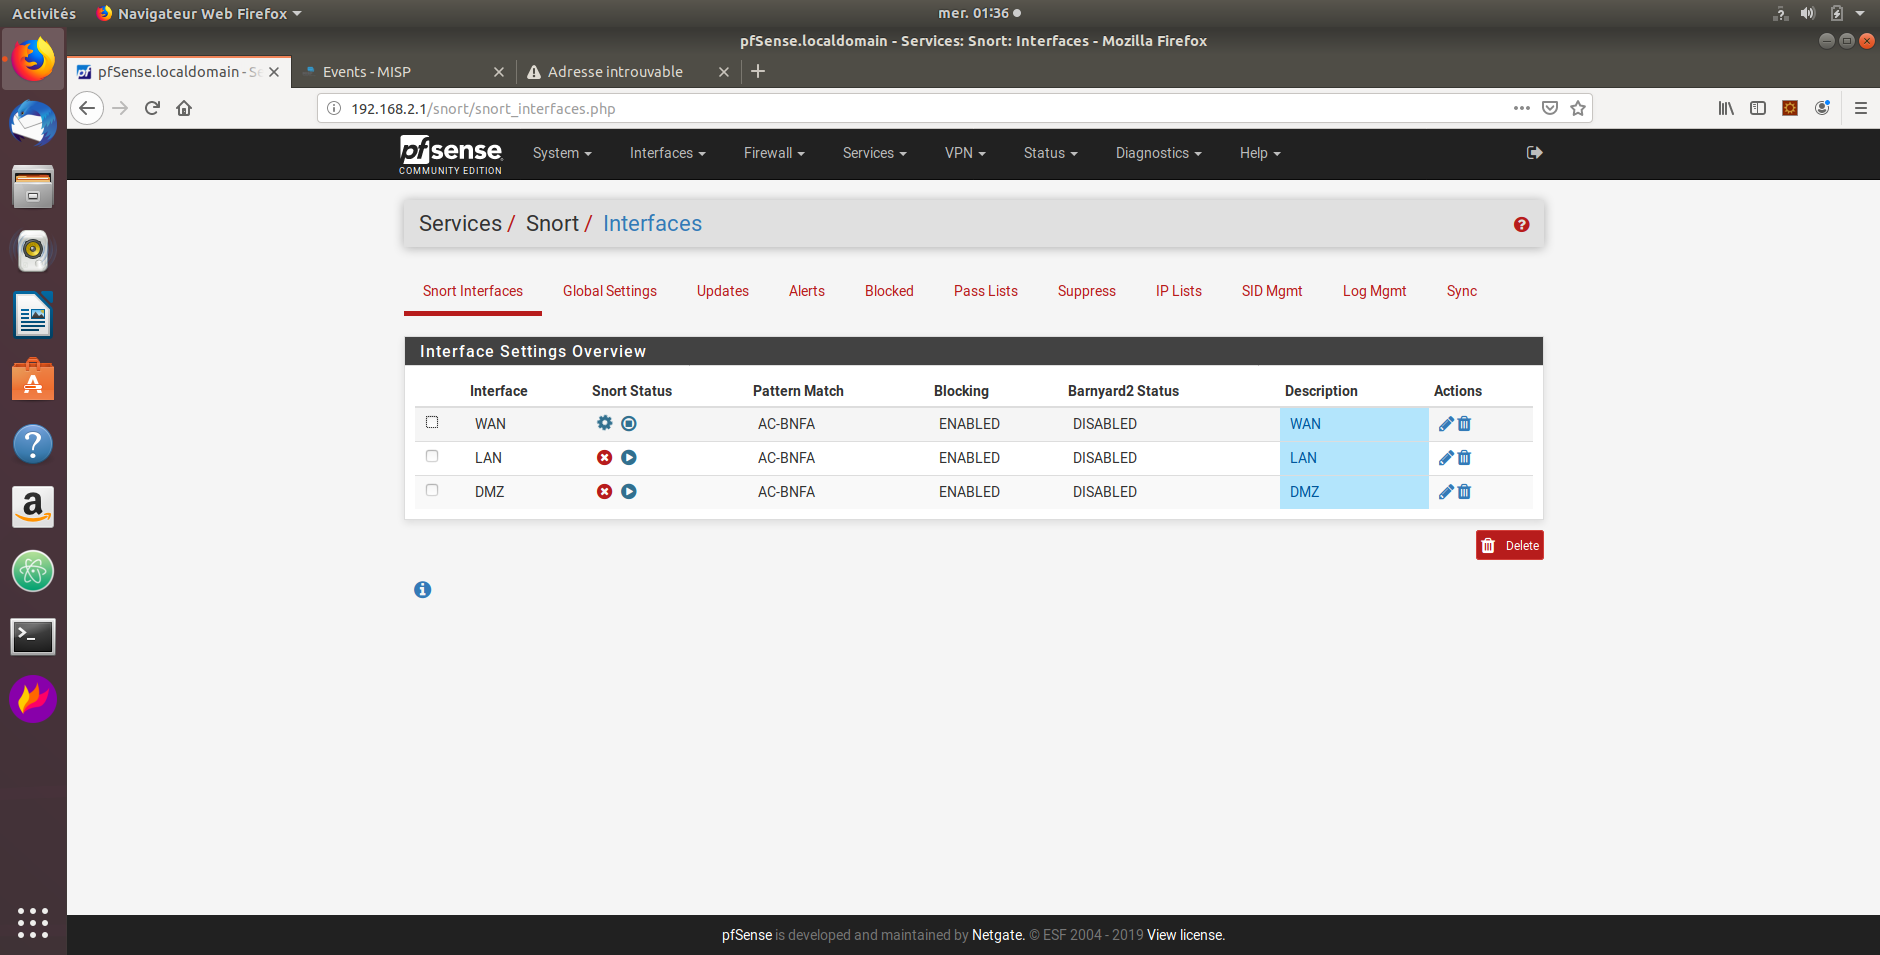
\includegraphics[scale=0.31]{MISP_Screenshots/Snort/16.png}
        \label{MISP_Screenshots/Snort/16}
        \caption{Lancement des trois interfaces nouvellement créées}
    \end{center}
\end{figure}
\FloatBarrier


\begin{figure}[h!]
    \begin{center}
        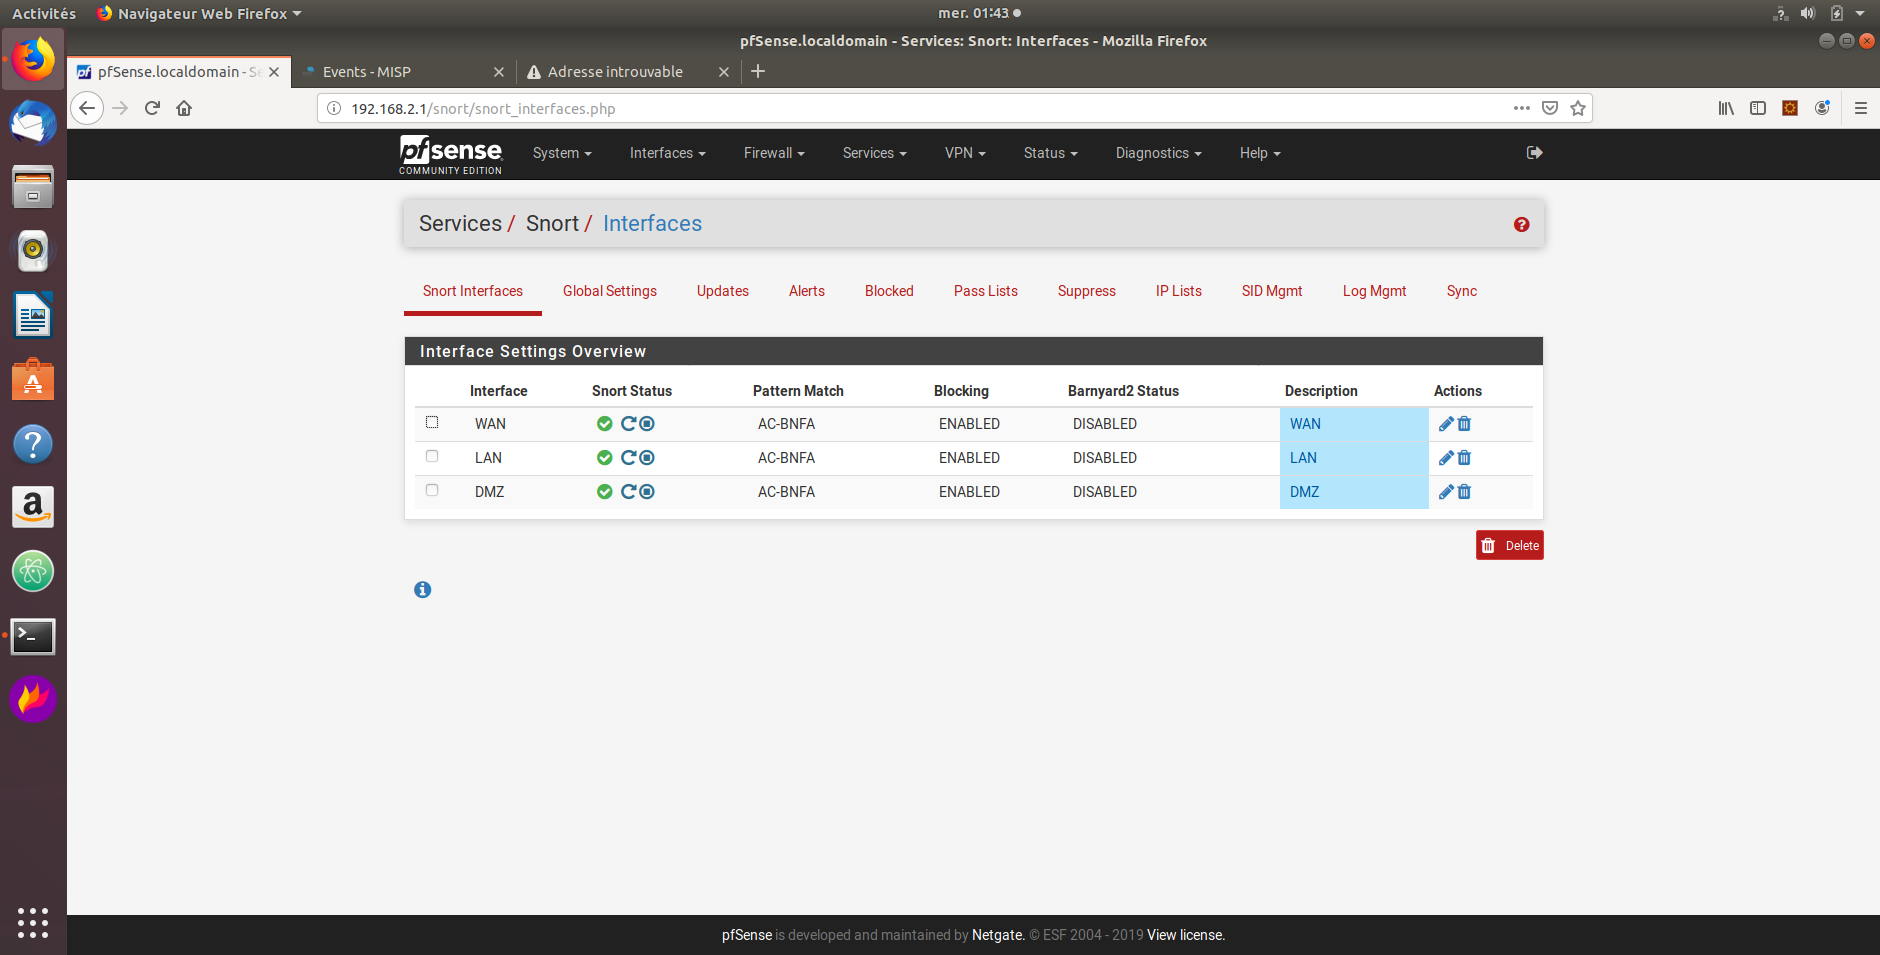
\includegraphics[scale=0.35]{MISP_Screenshots/Snort/17.png}
        \label{MISP_Screenshots/Snort/17}
        \caption{Affichage des trois nouvelles interfaces sur SNORT}
    \end{center}
\end{figure}
\FloatBarrier 
    